\documentclass{lecture}

\institute{Lehr- und Forschungsgebiet Kontinuumsmechanik}
\title{Vorlesung 2}
\author{Joshua Feld, 406718}
\course{Mechanik verformbarer Körper}
\professor{Itskov}
\semester{Sommersemester 2022}
\program{CES (Bachelor)}

\begin{document}
    \maketitle


    \section*{Hauptspannungen}

    Mit den Gleichungen \(\textup{(6)}^1\) haben wir die Spannungen in Abhängigkeit eines Schnittwinkels \(\varphi\) ausgedrückt.
    Im Hinblick auf die Festigkeit- bzw. Versagensanalyse wirft sich die Frage auf, unter welchem Winkel diese Spannungen Extremalwerte annehmen und wie groß diese Werte sind.
    Die notwendige Bedingung des Extremums \(\frac{\d\sigma_\xi}{\d\varphi} = 0\) bzw. \(\frac{\d\sigma_\eta}{\d\varphi} = 0\) führt zu den Gleichungen
    \begin{equation}\label{eq:1}
        -\parentheses*{\sigma_x - \sigma_y}\sin\parentheses*{2\varphi^*} + 2\tau_{xy}\cos\parentheses*{2\varphi^*} = 2\tau_{\xi\eta} = 0,
    \end{equation}
    wobei \(\varphi^*\) den Winkel des maximalen bzw. der minimalen Normalspannung bezeichnet.
    Man stellt auch fest, das die zugehörige Schubspannung unter diesem Winkel verschwindet.
    Dieser Winkel ergibt sich somit zu
    \begin{equation}\label{eq:2}
        \tan\parentheses*{2\varphi^*} = \frac{2\tau_{xy}}{\sigma_x - \sigma_y}.
    \end{equation}
    Da die Tangensfunktion \(\pi\)-periodisch ist, gilt \(\tan\parentheses*{2\varphi^*} = \tan\parentheses*{2\parentheses*{\varphi^* + \frac{\pi}{2}}}\).
    Somit ist \eqref{eq:2} für zwei senkrecht aufeinander stehende Schnittrichtungen \(\varphi^*\) und \(\varphi^* + \frac{\pi}{2}\) erfüllt, welche als Hauptrichtungen bezeichnet werden.
    Die zugehörigen Normalspannungen sind dann durch \(\textup{(6)}^1\) gegeben.
    Sie werden als Hauptspannungen \(\sigma_1\) und \(\sigma_2\) bezeichnet.
    Mithilfe der folgenden trigonometrischen Zusammenhänge
    \begin{align*}
        \cos\parentheses*{2\varphi^*} &= \frac{1}{\sqrt{1 + \tan^2\parentheses*{2\varphi^*}}} = \frac{\sigma_x - \sigma_y}{\sqrt{\parentheses*{\sigma_x - \sigma_y}^2 + 4\tau_{xy}^2}},\\
        \sin\parentheses*{2\varphi^*} &= \frac{\tan\parentheses*{2\varphi^*}}{\sqrt{1 + \tan^2\parentheses*{2\varphi^*}}} = \frac{2\tau_{xy}}{\sqrt{\parentheses*{\sigma_x - \sigma_y}^2 + 4\tau_{xy}^2}}
    \end{align*}
    erhält man somit
    \[
        \sigma_{1, 2} = \frac{1}{2}\parentheses*{\sigma_x + \sigma_y} \pm \frac{\frac{1}{2}\parentheses*{\sigma_x - \sigma_y}^2}{\sqrt{\parentheses*{\sigma_x - \sigma_y}^2 + 4\tau_{xy}^2}} \pm \frac{2\tau_{xy}^2}{\sqrt{\parentheses*{\sigma_x - \sigma_y}^2 + 4\tau_{xy}^2}}
    \]
    und schließlich
    \begin{equation}\label{eq:3}
        \sigma_{1, 2} = \frac{\sigma_x + \sigma_y}{2} \pm \sqrt{\parentheses*{\frac{\sigma_x - \sigma_y}{2}}^2 + \tau_{xy}^2}.
    \end{equation}
    Normalerweise werden die Hauptspannungen nach ihrer Größe nummeriert, so dass \(\sigma_1 > \sigma_2\).
    Wie bereits erwähnt verschwinden die Schubspannungen auf den zu den Hauptrichtungen orthogonalen Schnitten laut \eqref{eq:1}.
    Des Weiteren wird ein \(1, 2\)-Koordinatensystem, dessen Achsen mit den Hauptspannungsrichtungen übereinstimmen, als Hauptachsensystem bezeichnet.
    Dieses Koordinatensystem ist in der folgenden Abbildung illustriert.
    \begin{center}
        \begin{tikzpicture}
            \draw (0,0) rectangle (2,2);
            \draw[->] (-.1,1.25) -- (-.1,.75);
            \draw[->] (-.2,1) -- (-.7,1);
            \draw[->] (1.25,-.1) -- (.75,-.1);
            \draw[->] (1,-.2) -- (1,-.7);
            \draw[->] (2.1,.75) -- (2.1,1.25) node[right] {\(\tau_{xy}\)};
            \draw[->] (2.2,1) -- (2.7,1) node[right] {\(\sigma_x\)};
            \draw[->] (.75,2.1) -- (1.25,2.1) node[above right] {\(\tau_{xy}\)};
            \draw[->] (1,2.2) -- (1,2.7) node[right] {\(\sigma_y\)};
            \draw[->] (-.7,-.7) -- (-.2,-.7) node[right] {\(x\)};
            \draw[->] (-.7,-.7) -- (-.7,-.2) node[right] {\(y\)};
        \end{tikzpicture}
        \hspace{1cm}
        \begin{tikzpicture}
            \begin{scope}[rotate=20]
                \draw[->] (0,0) -- (3,0) coordinate (B) node[right] {\(1\)};
                \draw[->] (0,0) -- (0,3) node[right] {\(2\)};
                \draw (0,0) rectangle (2,2);
                \draw[->] (-.2,1) -- (-.7,1);
                \draw[->] (1,-.2) -- (1,-.7);
                \draw[->] (2.2,1) -- (2.7,1) node[right] {\(\sigma_1\)};
                \draw[->] (1,2.2) -- (1,2.7) node[above] {\(\sigma_2\)};
            \end{scope}
            \draw[dashed] (0,0) coordinate (O) -- (2.5,0) coordinate (A);
            \pic[draw,->,"$\varphi^*$",angle radius=2.3cm,angle eccentricity=1.15] {angle=A--O--B};
        \end{tikzpicture}
        \hspace{1cm}
        \begin{tikzpicture}
            \begin{scope}[rotate=65]
                \coordinate (B) at (2,0);
                \draw (0,0) rectangle (2,2);
                \draw[->] (-.1,1.25) -- (-.1,.75);
                \draw[->] (-.2,1) -- (-.7,1);
                \draw[->] (1.25,-.1) -- (.75,-.1);
                \draw[->] (1,-.2) -- (1,-.7);
                \draw[->] (2.1,.75) -- (2.1,1.25) node[above] {\(\tau_{\text{max}}\)};
                \draw[->] (2.2,1) -- (2.7,1) node[right] {\(\sigma_m\)};
                \draw[->] (.75,2.1) -- (1.25,2.1) node[above left] {\(\tau_{\text{max}}\)};
                \draw[->] (1,2.2) -- (1,2.7) node[left] {\(\sigma_m\)};
            \end{scope}
            \draw[dashed] (0,0) coordinate (O) -- (1,0) coordinate (A);
            \pic[draw,->] {angle=A--O--B};
            \node[anchor=north] at (.25,0) {\(\varphi^{**} = \varphi^* + \frac{\pi}{4}\)};
        \end{tikzpicture}
    \end{center}
    
    Analog zu den Extremalwerten der Normalspannung bestimmt man auch die maximale bzw. minimale Schubspannung und die zugehörigen Schnittrichtungen.
    Hierzu zieht man die Bedingung \(\frac{\d\tau_{\xi\eta}}{\d\varphi} = 0\) heran.
    Daraus folgt
    \[
        -\parentheses*{\sigma_x - \sigma_y}\cos\parentheses*{2\varphi^{**}} - 2\tau_{xy}\sin\parentheses*{2\varphi^{**}} = 0,
    \]
    wobei \(\varphi^{**}\) den Winkel dieser Schubrichtungen bezeichnet.
    Somit
    \begin{equation}\label{eq:4}
        \tan\parentheses*{2\varphi^{**}} = -\frac{\sigma_x - \sigma_y}{2\tau_{xy}}.
    \end{equation}
    Aus dem Vergleich von \eqref{eq:2} und \eqref{eq:4} erkennt man, dass
    \[
        \tan\parentheses*{2\varphi^{**}} = -\frac{1}{\tan\parentheses*{2\varphi^*}}.
    \]
    Somit ist die Richtung der extremalen Schubspannungen unter dem Winkel \(45^\circ\) zu den Hauptspannungen geneigt (siehe vorherige Abbildung).
    Die Extremalwerte der Schubspannungen bezeichnet man als Hauptschubspannungen.
    Diese ergeben sich durch Einsetzen von \eqref{eq:4} in \(\textup{(6)}^1\) zu
    \[
        \tau_{\text{max}} = \pm\sqrt{\parentheses*{\frac{\sigma_x - \sigma_y}{2}}^2 + \tau_{xy}^2}.
    \]
    Somit besteht der folgende Zusammenhang mit den Hauptspannungen \eqref{eq:3}
    \[
        \tau_{\text{max}} = \pm\frac{1}{2}\parentheses*{\sigma_1 - \sigma_2}.
    \]
    Auf den Schnitten mit den extremalen Schubspannungen ist die Normalspannung im Allgemeinen von Null verschieden.
    Diese Normalspannung ergibt sich durch Einsetzen von \(\varphi^{**}\) in \(\textup{(6)}^1\) zu
    \begin{equation}\label{eq:5}
        \sigma_m = \frac{1}{2}\parentheses*{\sigma_x + \sigma_y} = \frac{1}{2}\parentheses*{\sigma_1 + \sigma_2}.
    \end{equation}


    \section*{Mohrscher Spannungskreis}

    Der Mohrsche Spannungskreis ist eine geometrische Darstellung der Transformationsgleichungen \(\textup{(6)}^1\).
    Nach ihrer Umordnung erhält man
    \begin{align*}
        \sigma_\xi - \frac{1}{2}\parentheses*{\sigma_x + \sigma_y} &= \frac{1}{2}\parentheses*{\sigma_x - \sigma_y}\cos\parentheses*{2\varphi} + \tau_{xy}\sin\parentheses*{2\varphi},\\
        \tau_{\xi\eta} &= -\frac{1}{2}\parentheses*{\sigma_x - \sigma_y}\sin\parentheses*{2\varphi} + \tau_{xy}\cos\parentheses*{2\varphi}.
    \end{align*}
    Quadrieren und Addieren ergibt schließlich
    \begin{equation}\label{eq:6}
        \parentheses*{\sigma_\xi - \frac{1}{2}\parentheses*{\sigma_x + \sigma_y}}^2 + \tau_{\xi\eta}^2 = \parentheses*{\frac{\sigma_x - \sigma_y}{2}}^2 + \tau_{xy}^2.
    \end{equation}
    Unter Ausnutzung von \eqref{eq:5} und mithilfe der Abkürzung
    \begin{equation}\label{eq:7}
        r^2 = \parentheses*{\frac{\sigma_x - \sigma_y}{2}}^2 + \tau_{xy}^2
    \end{equation}
    können wir \eqref{eq:6} wie folgt umschreiben
    \[
        \parentheses*{\sigma - \sigma_m}^2 + \tau^2 = r^2,
    \]
    wobei die Indizes von nun an ausgelassen werden können.
    Dies ist die Gleichung eines Kreises in der \(\sigma, \tau\)-Ebene mit dem Mittelpunkt \(\parentheses*{\sigma_m, 0}\) und Radius \(r\).
    Dieser Kreis wird Mohrscher Spannungskreis bezeichnet.

    Die Lage des Kreises wird durch zwei Werte \(\sigma_m\) \eqref{eq:5} und \(r\) \eqref{eq:7} bestimmt, die somit Spannungsinvarianten darstellen.
    Diese können durch die Spur und die Determinante des zweidimensionalen Spannungstensors
    \begin{align*}
        I_1 &= \sigma_x + \sigma_y,\\
        I_2 &= \sigma_x \sigma_y - \tau_{xy}^2
    \end{align*}
    eindeutig ausgedrückt werden.
    In der Tat erhält man durch Umschreiben von \eqref{eq:7}
    \begin{align*}
        r^2 &= r^2 + \sigma_x \sigma_y - \sigma_x \sigma_y\\
        &= \parentheses*{\frac{\sigma_x + \sigma_y}{2}}^2 + \tau_{xy}^2 - \sigma_x \sigma_y\\
        &= \frac{1}{4}\parentheses*{I_1^2 - 4I_2}.
    \end{align*}
    Ein Kreis kann eindeutig durch drei Punkte festgelegt werden.
    Die Spannungen auf zwei zueinander senkrechten Ebenen \(\sigma_x\), \(\sigma_y\) und \(\tau_{xy}\) liefern allerdings lediglich zwei Punkte.
    Die Tatsache, dass diese Ebenen orthogonal zueinander sind, liefert aber den Kreismittelpunkt \(\parentheses*{\sigma_m, 0}\).
    Damit reichen diese zwei Punkte, um den Spannungskreis eindeutig zu definieren.
    Im Folgenden wird die Vorgehensweise zur Konstruktion des Mohrschen Spannungskreises anhand der bekannten Werten von \(\sigma_x\), \(\sigma_y\) und \(\tau_{xy}\) skizziert.
    \begin{enumerate}
        \item Auf der \(\sigma\)-Achse werden \(\sigma_x\) und \(\sigma_y\) unter Beachtung des Vorzeichens eingetragen.
        \item \(\tau_{xy}\) vorzeichenrichtig über \(\sigma_x\) (Punkt \(P\)) und mit umgedrehtem Vorzeichen über \(\sigma_y\) (Punkt \(P'\)) eintragen.
        \item Punkte \(P\) und \(P'\) verbinden.
        Der Kreismittelpunkt ergibt sich als Schnittpunkt mit der \(\sigma\)-Achse.
        \item Spannungskreis mit diesem Mittelpunkt durch die Punkte \(P\) und \(P'\) zeichnen.
    \end{enumerate}
    \begin{center}
        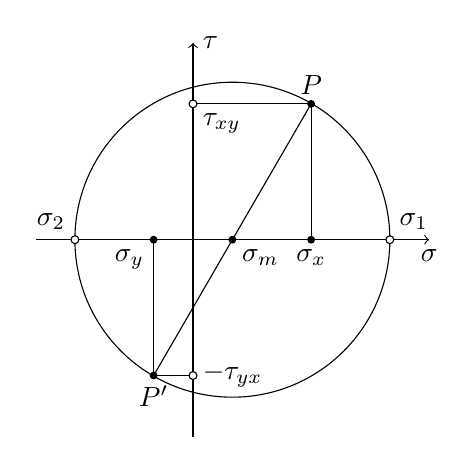
\begin{tikzpicture}
            \draw (.5,0) circle (2cm);
            \draw[->] (-2,0) -- (3,0) node[below] {\(\sigma\)};
            \draw[->] (0,-2.5) -- (0,2.5) node[right] {\(\tau\)};
            \fill (.5,0) circle (.5mm) node[below right] {\(\sigma_m\)};
            \fill (1.5,0) circle (.5mm) node[below] {\(\sigma_x\)};
            \fill (-.5,0) circle (.5mm) node[below left] {\(\sigma_y\)};
            \draw[fill=white] (2.5,0) circle (.5mm) node[above right] {\(\sigma_1\)};
            \draw[fill=white] (-1.5,0) circle (.5mm) node[above left] {\(\sigma_2\)};
            \draw (1.5,0) -- (1.5,1.725);
            \draw (-.5,0) -- (-.5,-1.725);
            \draw (-.5,-1.725) -- (1.5,1.725);
            \draw (1.5,1.725) -- (0,1.725);
            \draw[fill=white] (0,1.725) circle (.5mm) node[below right] {\(\tau_{xy}\)};
            \draw (-.5,-1.725) -- (0,-1.725);
            \draw[fill=white] (0,-1.725) circle (.5mm) node[right] {\(-\tau_{yx}\)};
            \fill (-.5,-1.725) circle (.5mm) node[below] {\(P'\)};
            \fill (1.5,1.725) circle (.5mm) node[above] {\(P\)};
        \end{tikzpicture}
    \end{center}
    Der Mohrsche Spannungskreis (siehe folgende Abbildung) liefert viele wichtige Informationen bezüglich des Spannungszustandes.
    Zum einen lassen sich daraus die Hauptspannungen \(\sigma_1, \sigma_2\) sowie die maximale Schubspannung \(\tau_{\text{max}}\) leicht ablesen.
    Die Winkel \(2\varphi^*\) \eqref{eq:2} und \(2\varphi^{**}\) \eqref{eq:4} ergeben sich dabei als die Winkel zwischen dem Radius zum Punkt \(P\) und der horizontalen bzw. vertikalen Achse.
    Somit erkennt man unmittelbar, dass sich diese Winkel um \(\frac{\pi}{2}\) unterscheiden.
    Zum anderen kann man die Spannungen in einem um den Winkel \(\varphi\) geneigten Koordinatensystem bestimmen.
    Hierzu wird der Radius um den Winkel \(2\varphi\) im Uhrzeigersinn gedreht.
    Entgegen der üblichen Vorzeichenregel ist es eine positive Winkelrichtung für den Mohrschen Spannungskreis.
    So gelangt man von den Punkten \(P\) und \(P'\) zu den Punkten \(Q\) bzw. \(Q'\) mit den Koordinaten \(\sigma_\xi\), \(\sigma_\eta\) und \(\tau_{\xi\eta}\).
    \begin{center}
        \begin{tikzpicture}
            \draw[->] (-5,0) -- (5,0) coordinate (sigma) node[below] {\(\sigma\)};
            \draw[<->] (-5,-4.5) -- (-5,4.5) node[right] {\(\tau\)};
            \draw (0,0) circle (3.5cm);
            \draw[dashed] (0,3.5) -- (-5,3.5) node[left] {\(\tau_{\text{max}}\)};
            \draw[dashed] (0,-3.5) -- (-5,-3.5) node[left] {\(\tau_{\text{max}}\)};
            \draw (0,-3.5) coordinate (tau_max) -- (0,0) coordinate (sigma_m) -- (0,3.5) node[midway,right] {\(r\)};
            \draw[dashed] (-2.5,0) -- (-2.5,-2.45);
            \draw[dashed] (-2.5,-2.45) -- (2.5,2.45);
            \draw[dashed] (2.5,0) -- (2.5,2.45) node[pos=.2,right] {\(\tau_{\eta\xi}\)};
            \draw (-1.25,0) -- (-1.25,-3.275);
            \draw (1.25,0) -- (1.25,3.275) node[pos=.875,right] {\(\tau_{xy}\)};
            \draw (-1.25,-3.275) -- (1.25,3.275);
            \draw[fill=white] (0,-3.5) circle (.5mm);
            \draw[fill=white] (0,3.5) circle (.5mm);
            \draw[fill=white] (-3.5,0) circle (.5mm) node[below left] {\(\sigma_2\)};
            \draw[fill=white] (-2.5,0) circle (.5mm) node[below right] {\(\sigma_\eta\)};
            \draw[fill=white] (-1.25,0) circle (.5mm) node[below right] {\(\sigma_y\)};
            \fill (0,0) circle (.5mm) node[below right] {\(\sigma_m\)};
            \draw[fill=white] (1.25,0) circle (.5mm) node[below] {\(\sigma_x\)};
            \draw[fill=white] (2.5,0) circle (.5mm) node[below] {\(\sigma_\xi\)};
            \draw[fill=white] (3.5,0) circle (.5mm) node[below right] {\(\sigma_1\)};
            \draw[fill=white] (-2.5,-2.45) circle (.5mm) node[below left] {\(Q'\)};
            \draw[fill=white] (2.5,2.45) coordinate (Q) circle (.5mm) node[above right] {\(Q\)};
            \draw[fill=white] (-1.25,-3.275) circle (.5mm) node[above right] {\(P'\)};
            \draw[fill=white] (1.25,3.275) coordinate (P) circle (.5mm) node[above right] {\(P\)};
            \pic[draw,<-,"$2\varphi$",angle radius=2.5cm,angle eccentricity=1.15] {angle=Q--sigma_m--P};
            \pic[draw,<-,"$2\varphi^*$",angle radius=2cm,angle eccentricity=1.25] {angle=sigma--sigma_m--P};
            \pic[draw,<-,angle radius=1cm] {angle=tau_max--sigma_m--P};
            \node at (1,-1) {\(2\varphi^{**}\)};
            \pic[draw,<-,"$2 \cdot 45^\circ$",angle radius=2.25cm,angle eccentricity=1.2] {angle=tau_max--sigma_m--sigma};
        \end{tikzpicture}
    \end{center}
    Nun betrachten wir den Mohrschen Spannungskreis für einige wichtige Sonderfälle des Spannungszustandes.
    \begin{itemize}
        \item \emph{Einachsiger Zug} entsteht im klassischen Zugversuch, der zur Charakterisierung der Materialeigenschaften durchgeführt wird.
        Dabei ist die Zugspannung gleich der Normalspannung in \(x\)-Richtung (\(\sigma_x = \sigma_0\)).
        Die Normalspannung in \(y\)-Richtung sowie die Schubspannung fallen weg (\(\sigma_y = \tau_{xy} = 0\)).
        Man erkennt auch, dass \(\sigma_1 = \sigma_0\) und \(\sigma_2 = 0\).
        Die maximale Schubspannung \(\tau_{\text{max}} = \frac{\sigma_0}{2}\) entsteht in den Schnitten, die zur Zugachse um den Winkel \(45^\circ\) geneigt sind.
        \begin{center}
            \begin{tikzpicture}
                \draw[->] (0,0) -- (3,0) node[above] {\(x\)};
                \draw[->] (0,0) -- (0,3) node[left] {\(y\)};
                \draw (0,0) rectangle (2,2);
                \draw[->] (-.2,1) -- (-.7,1) node[below] {\(\sigma_0\)};
                \draw[->] (2.2,1) -- (2.7,1) node[below] {\(\sigma_0\)};
            \end{tikzpicture}\hspace{2cm}
            \begin{tikzpicture}
                \draw[->] (-1.5,0) -- (2.5,0) node[below] {\(\sigma\)};
                \draw[->] (0,-1.5) -- (0,2.5) node[left] {\(\tau\)};
                \draw (1,0) circle (1cm);
                \draw[dashed] (1,1) -- (1,-1);
                \fill (1,1) circle (.5mm) node[above] {\(\tau_{\text{max}}\)};
                \fill (1,-1) circle (.5mm);
                \fill (0,0) circle (.5mm) node[above left] {\(\sigma_y\)};
                \fill (2,0) circle (.5mm) node[above right] {\(\sigma_x = \sigma_0\)};
            \end{tikzpicture}
        \end{center}
        \item \emph{Einfacher Schub} entsteht beispielsweise bei Torsion.
        Für den einfachen Schub ist es charakteristisch, dass keine Normalspannungen (\(\sigma_x = \sigma_y = 0\)) sondern nur Schubspannungen auftreten.
        Die maximale Schubspannung ist in diesem Fall gleich der angreifenden Schubspannung (\(\tau_{\text{max}} = \tau_0\)) und stimmt mit den Hauptspannungen (bis auf das Vorzeichen) überein: \(\sigma_1 = -\sigma_2 = \tau_0\).
        Die entstehenden Hauptspannungen und dazugehörigen Hauptrichtungen sind in dem dritten Bild dargestellt.
        \begin{center}
            \begin{tikzpicture}
                \draw[->] (0,0) -- (3,0) node[above] {\(x\)};
                \draw[->] (0,0) -- (0,3) node[left] {\(y\)};
                \draw (0,0) rectangle (2,2);
                \draw[->] (-.1,1.25) -- (-.1,.75);
                \draw[->] (1.25,-.1) -- (.75,-.1);
                \draw[->] (.75,2.1) -- (1.25,2.1) node[above] {\(\tau_0\)};
                \draw[->] (2.1,.75) -- (2.1,1.25) node[right] {\(\tau_0\)};
            \end{tikzpicture}\hspace{1cm}
            \begin{tikzpicture}
                \draw[->] (-1.5,0) -- (2.5,0) node[below] {\(\sigma\)};
                \draw[->] (0,-1.5) -- (0,2.5) node[left] {\(\tau\)};
                \draw (0,0) circle (1cm);
                \fill (0,1) circle (.5mm) node[above right] {\(\tau_0\)};
                \fill (0,-1) circle (.5mm);
                \fill (-1,0) circle (.5mm) node[above left] {\(\sigma_2\)};
                \fill (1,0) circle (.5mm) node[above right] {\(\sigma_1\)};
            \end{tikzpicture}
            \hspace{1cm}
            \begin{tikzpicture}
                \begin{scope}[rotate=45]
                    \draw (-1,0) coordinate (O) -- (0,0) coordinate (A);
                    \draw (0,0) rectangle (2,2);
                    \draw[->] (1,-.7) node[right] {\(\tau_0\)} -- (1,-.2);
                    \draw[->] (2.2,1) -- (2.7,1) node[above] {\(\tau_0\)};
                    \draw[->] (1,2.7) node[above] {\(\tau_0\)} -- (1,2.2);
                    \draw[->] (-.2,1) -- (-.7,1) node[left] {\(\tau_0\)};
                \end{scope}
                \draw (O) -- (.7,-.7) coordinate (B);
                \pic[draw,->,"$45^\circ$",angle radius=.75cm,angle eccentricity=1.45] {angle=B--O--A};
            \end{tikzpicture}
        \end{center}
        \item \emph{Hydrostatischer Druck} entsteht beispielsweise unter Wasser, wobei von allen Seiten die gleiche Spannung \(p\) aufgebracht wird.
        In diesem Fall sind alle Normalspannungen gleich dieser Druckspannung (\(\sigma_x = \sigma_y = -p\)) und die Schubspannungskomponente ist gleich Null (\(\tau_{xy} = 0\)).
        Der Mohrsche Spannungskreis entartet sich zu einem Punkt in der \(\tau-\sigma\) Ebene, so dass \(\tau_{\text{max}} = 0\).
        \begin{center}
            \begin{tikzpicture}
                \draw[->] (0,0) -- (3,0) node[above] {\(x\)};
                \draw[->] (0,0) -- (0,3) node[left] {\(y\)};
                \draw (0,0) rectangle (2,2);
                \draw[->] (1,2.7) node[right] {\(p\)} -- (1,2.2);
                \draw[->] (2.7,1) node[below] {\(p\)} -- (2.2,1);
                \draw[->] (1,-.7) -- (1,-.2);
                \draw[->] (-.7,1) -- (-.2,1);
            \end{tikzpicture}\hspace{2cm}
            \begin{tikzpicture}
                \draw[->] (-2,0) -- (1,0) node[below] {\(\sigma\)};
                \draw[->] (0,-1.5) -- (0,2.5) node[left] {\(\tau\)};
                \fill (-1,0) circle (.5mm) node[below] {\(p\)};
                \node[anchor=east] at (0,-1) {\(\sigma_1 = \sigma_2 = -p\)};
            \end{tikzpicture}
        \end{center}
    \end{itemize}
\end{document}
